
%% bare_conf.tex
%% V1.3
%% 2007/01/11
%% by Michael Shell
%% See:
%% http://www.michaelshell.org/
%% for current contact information.
%%
%% This is a skeleton file demonstrating the use of IEEEtran.cls
%% (requires IEEEtran.cls version 1.7 or later) with an IEEE conference paper.
%%
%% Support sites:
%% http://www.michaelshell.org/tex/ieeetran/
%% http://www.ctan.org/tex-archive/macros/latex/contrib/IEEEtran/
%% and
%% http://www.ieee.org/

%%*************************************************************************
%% Legal Notice:
%% This code is offered as-is without any warranty either expressed or
%% implied; without even the implied warranty of MERCHANTABILITY or
%% FITNESS FOR A PARTICULAR PURPOSE! 
%% User assumes all risk.
%% In no event shall IEEE or any contributor to this code be liable for
%% any damages or losses, including, but not limited to, incidental,
%% consequential, or any other damages, resulting from the use or misuse
%% of any information contained here.
%%
%% All comments are the opinions of their respective authors and are not
%% necessarily endorsed by the IEEE.
%%
%% This work is distributed under the LaTeX Project Public License (LPPL)
%% ( http://www.latex-project.org/ ) version 1.3, and may be freely used,
%% distributed and modified. A copy of the LPPL, version 1.3, is included
%% in the base LaTeX documentation of all distributions of LaTeX released
%% 2003/12/01 or later.
%% Retain all contribution notices and credits.
%% ** Modified files should be clearly indicated as such, including  **
%% ** renaming them and changing author support contact information. **
%%
%% File list of work: IEEEtran.cls, IEEEtran_HOWTO.pdf, bare_adv.tex,
%%                    bare_conf.tex, bare_jrnl.tex, bare_jrnl_compsoc.tex
%%*************************************************************************

% *** Authors should verify (and, if needed, correct) their LaTeX system  ***
% *** with the testflow diagnostic prior to trusting their LaTeX platform ***
% *** with production work. IEEE's font choices can trigger bugs that do  ***
% *** not appear when using other class files.                            ***
% The testflow support page is at:
% http://www.michaelshell.org/tex/testflow/



% Note that the a4paper option is mainly intended so that authors in
% countries using A4 can easily print to A4 and see how their papers will
% look in print - the typesetting of the document will not typically be
% affected with changes in paper size (but the bottom and side margins will).
% Use the testflow package mentioned above to verify correct handling of
% both paper sizes by the user's LaTeX system.
%
% Also note that the "draftcls" or "draftclsnofoot", not "draft", option
% should be used if it is desired that the figures are to be displayed in
% draft mode.
%
\documentclass[conference]{IEEEtran}
% Add the compsoc option for Computer Society conferences.
%
% If IEEEtran.cls has not been installed into the LaTeX system files,
% manually specify the path to it like:
% \documentclass[conference]{../sty/IEEEtran}





% Some very useful LaTeX packages include:
% (uncomment the ones you want to load)


% *** MISC UTILITY PACKAGES ***
%
%\usepackage{ifpdf}
% Heiko Oberdiek's ifpdf.sty is very useful if you need conditional
% compilation based on whether the output is pdf or dvi.
% usage:
% \ifpdf
%   % pdf code
% \else
%   % dvi code
% \fi
% The latest version of ifpdf.sty can be obtained from:
% http://www.ctan.org/tex-archive/macros/latex/contrib/oberdiek/
% Also, note that IEEEtran.cls V1.7 and later provides a builtin
% \ifCLASSINFOpdf conditional that works the same way.
% When switching from latex to pdflatex and vice-versa, the compiler may
% have to be run twice to clear warning/error messages.
\usepackage{graphicx}





% *** CITATION PACKAGES ***
%
%\usepackage{cite}
% cite.sty was written by Donald Arseneau
% V1.6 and later of IEEEtran pre-defines the format of the cite.sty package
% \cite{} output to follow that of IEEE. Loading the cite package will
% result in citation numbers being automatically sorted and properly
% "compressed/ranged". e.g., [1], [9], [2], [7], [5], [6] without using
% cite.sty will become [1], [2], [5]--[7], [9] using cite.sty. cite.sty's
% \cite will automatically add leading space, if needed. Use cite.sty's
% noadjust option (cite.sty V3.8 and later) if you want to turn this off.
% cite.sty is already installed on most LaTeX systems. Be sure and use
% version 4.0 (2003-05-27) and later if using hyperref.sty. cite.sty does
% not currently provide for hyperlinked citations.
% The latest version can be obtained at:
% http://www.ctan.org/tex-archive/macros/latex/contrib/cite/
% The documentation is contained in the cite.sty file itself.






% *** GRAPHICS RELATED PACKAGES ***
%
\ifCLASSINFOpdf
  % \usepackage[pdftex]{graphicx}
  % declare the path(s) where your graphic files are
  % \graphicspath{{../pdf/}{../jpeg/}}
  % and their extensions so you won't have to specify these with
  % every instance of \includegraphics
  % \DeclareGraphicsExtensions{.pdf,.jpeg,.png}
\else
  % or other class option (dvipsone, dvipdf, if not using dvips). graphicx
  % will default to the driver specified in the system graphics.cfg if no
  % driver is specified.
  % \usepackage[dvips]{graphicx}
  % declare the path(s) where your graphic files are
  % \graphicspath{{../eps/}}
  % and their extensions so you won't have to specify these with
  % every instance of \includegraphics
  % \DeclareGraphicsExtensions{.eps}
\fi
% graphicx was written by David Carlisle and Sebastian Rahtz. It is
% required if you want graphics, photos, etc. graphicx.sty is already
% installed on most LaTeX systems. The latest version and documentation can
% be obtained at: 
% http://www.ctan.org/tex-archive/macros/latex/required/graphics/
% Another good source of documentation is "Using Imported Graphics in
% LaTeX2e" by Keith Reckdahl which can be found as epslatex.ps or
% epslatex.pdf at: http://www.ctan.org/tex-archive/info/
%
% latex, and pdflatex in dvi mode, support graphics in encapsulated
% postscript (.eps) format. pdflatex in pdf mode supports graphics
% in .pdf, .jpeg, .png and .mps (metapost) formats. Users should ensure
% that all non-photo figures use a vector format (.eps, .pdf, .mps) and
% not a bitmapped formats (.jpeg, .png). IEEE frowns on bitmapped formats
% which can result in "jaggedy"/blurry rendering of lines and letters as
% well as large increases in file sizes.
%
% You can find documentation about the pdfTeX application at:
% http://www.tug.org/applications/pdftex





% *** MATH PACKAGES ***
%
%\usepackage[cmex10]{amsmath}
% A popular package from the American Mathematical Society that provides
% many useful and powerful commands for dealing with mathematics. If using
% it, be sure to load this package with the cmex10 option to ensure that
% only type 1 fonts will utilized at all point sizes. Without this option,
% it is possible that some math symbols, particularly those within
% footnotes, will be rendered in bitmap form which will result in a
% document that can not be IEEE Xplore compliant!
%
% Also, note that the amsmath package sets \interdisplaylinepenalty to 10000
% thus preventing page breaks from occurring within multiline equations. Use:
%\interdisplaylinepenalty=2500
% after loading amsmath to restore such page breaks as IEEEtran.cls normally
% does. amsmath.sty is already installed on most LaTeX systems. The latest
% version and documentation can be obtained at:
% http://www.ctan.org/tex-archive/macros/latex/required/amslatex/math/





% *** SPECIALIZED LIST PACKAGES ***
%
%\usepackage{algorithmic}
% algorithmic.sty was written by Peter Williams and Rogerio Brito.
% This package provides an algorithmic environment fo describing algorithms.
% You can use the algorithmic environment in-text or within a figure
% environment to provide for a floating algorithm. Do NOT use the algorithm
% floating environment provided by algorithm.sty (by the same authors) or
% algorithm2e.sty (by Christophe Fiorio) as IEEE does not use dedicated
% algorithm float types and packages that provide these will not provide
% correct IEEE style captions. The latest version and documentation of
% algorithmic.sty can be obtained at:
% http://www.ctan.org/tex-archive/macros/latex/contrib/algorithms/
% There is also a support site at:
% http://algorithms.berlios.de/index.html
% Also of interest may be the (relatively newer and more customizable)
% algorithmicx.sty package by Szasz Janos:
% http://www.ctan.org/tex-archive/macros/latex/contrib/algorithmicx/




% *** ALIGNMENT PACKAGES ***
%
%\usepackage{array}
% Frank Mittelbach's and David Carlisle's array.sty patches and improves
% the standard LaTeX2e array and tabular environments to provide better
% appearance and additional user controls. As the default LaTeX2e table
% generation code is lacking to the point of almost being broken with
% respect to the quality of the end results, all users are strongly
% advised to use an enhanced (at the very least that provided by array.sty)
% set of table tools. array.sty is already installed on most systems. The
% latest version and documentation can be obtained at:
% http://www.ctan.org/tex-archive/macros/latex/required/tools/


%\usepackage{mdwmath}
%\usepackage{mdwtab}
% Also highly recommended is Mark Wooding's extremely powerful MDW tools,
% especially mdwmath.sty and mdwtab.sty which are used to format equations
% and tables, respectively. The MDWtools set is already installed on most
% LaTeX systems. The lastest version and documentation is available at:
% http://www.ctan.org/tex-archive/macros/latex/contrib/mdwtools/


% IEEEtran contains the IEEEeqnarray family of commands that can be used to
% generate multiline equations as well as matrices, tables, etc., of high
% quality.


%\usepackage{eqparbox}
% Also of notable interest is Scott Pakin's eqparbox package for creating
% (automatically sized) equal width boxes - aka "natural width parboxes".
% Available at:
% http://www.ctan.org/tex-archive/macros/latex/contrib/eqparbox/





% *** SUBFIGURE PACKAGES ***
%\usepackage[tight,footnotesize]{subfigure}
% subfigure.sty was written by Steven Douglas Cochran. This package makes it
% easy to put subfigures in your figures. e.g., "Figure 1a and 1b". For IEEE
% work, it is a good idea to load it with the tight package option to reduce
% the amount of white space around the subfigures. subfigure.sty is already
% installed on most LaTeX systems. The latest version and documentation can
% be obtained at:
% http://www.ctan.org/tex-archive/obsolete/macros/latex/contrib/subfigure/
% subfigure.sty has been superceeded by subfig.sty.



%\usepackage[caption=false]{caption}
%\usepackage[font=footnotesize]{subfig}
% subfig.sty, also written by Steven Douglas Cochran, is the modern
% replacement for subfigure.sty. However, subfig.sty requires and
% automatically loads Axel Sommerfeldt's caption.sty which will override
% IEEEtran.cls handling of captions and this will result in nonIEEE style
% figure/table captions. To prevent this problem, be sure and preload
% caption.sty with its "caption=false" package option. This is will preserve
% IEEEtran.cls handing of captions. Version 1.3 (2005/06/28) and later 
% (recommended due to many improvements over 1.2) of subfig.sty supports
% the caption=false option directly:
%\usepackage[caption=false,font=footnotesize]{subfig}
%
% The latest version and documentation can be obtained at:
% http://www.ctan.org/tex-archive/macros/latex/contrib/subfig/
% The latest version and documentation of caption.sty can be obtained at:
% http://www.ctan.org/tex-archive/macros/latex/contrib/caption/




% *** FLOAT PACKAGES ***
%
%\usepackage{fixltx2e}
% fixltx2e, the successor to the earlier fix2col.sty, was written by
% Frank Mittelbach and David Carlisle. This package corrects a few problems
% in the LaTeX2e kernel, the most notable of which is that in current
% LaTeX2e releases, the ordering of single and double column floats is not
% guaranteed to be preserved. Thus, an unpatched LaTeX2e can allow a
% single column figure to be placed prior to an earlier double column
% figure. The latest version and documentation can be found at:
% http://www.ctan.org/tex-archive/macros/latex/base/



%\usepackage{stfloats}
% stfloats.sty was written by Sigitas Tolusis. This package gives LaTeX2e
% the ability to do double column floats at the bottom of the page as well
% as the top. (e.g., "\begin{figure*}[!b]" is not normally possible in
% LaTeX2e). It also provides a command:
%\fnbelowfloat
% to enable the placement of footnotes below bottom floats (the standard
% LaTeX2e kernel puts them above bottom floats). This is an invasive package
% which rewrites many portions of the LaTeX2e float routines. It may not work
% with other packages that modify the LaTeX2e float routines. The latest
% version and documentation can be obtained at:
% http://www.ctan.org/tex-archive/macros/latex/contrib/sttools/
% Documentation is contained in the stfloats.sty comments as well as in the
% presfull.pdf file. Do not use the stfloats baselinefloat ability as IEEE
% does not allow \baselineskip to stretch. Authors submitting work to the
% IEEE should note that IEEE rarely uses double column equations and
% that authors should try to avoid such use. Do not be tempted to use the
% cuted.sty or midfloat.sty packages (also by Sigitas Tolusis) as IEEE does
% not format its papers in such ways.





% *** PDF, URL AND HYPERLINK PACKAGES ***
%
%\usepackage{url}
% url.sty was written by Donald Arseneau. It provides better support for
% handling and breaking URLs. url.sty is already installed on most LaTeX
% systems. The latest version can be obtained at:
% http://www.ctan.org/tex-archive/macros/latex/contrib/misc/
% Read the url.sty source comments for usage information. Basically,
% \url{my_url_here}.





% *** Do not adjust lengths that control margins, column widths, etc. ***
% *** Do not use packages that alter fonts (such as pslatex).         ***
% There should be no need to do such things with IEEEtran.cls V1.6 and later.
% (Unless specifically asked to do so by the journal or conference you plan
% to submit to, of course. )


% correct bad hyphenation here
\hyphenation{op-tical net-works semi-conduc-tor}


\begin{document}
%
% paper title
% can use linebreaks \\ within to get better formatting as desired
\title{Social Testing: A Framework to support adoption of continuous delivery by Small Medium Enterprises.}


% author names and affiliations
% use a multiple column layout for up to three different
% affiliations
% author names and affiliations
% use a multiple column layout for up to three different
% affiliations
%\author{\IEEEauthorblockN{Michael Shell}
%\IEEEauthorblockA{School of Electrical and\\Computer Engineering\\
%Georgia Institute of Technology\\
%Atlanta, Georgia 30332--0250\\
%Email: http://www.michaelshell.org/contact.html}
%\and
%\IEEEauthorblockN{Homer Simpson}
%\IEEEauthorblockA{Twentieth Century Fox\\
%Springfield, USA\\
%Email: homer@thesimpsons.com}
%\and
%\IEEEauthorblockN{James Kirk\\ and Montgomery Scott}
%\IEEEauthorblockA{Starfleet Academy\\
%San Francisco, California 96678-2391\\
%Telephone: (800) 555--1212\\
%Fax: (888) 555--1212}}

% conference papers do not typically use \thanks and this command
% is locked out in conference mode. If really needed, such as for
% the acknowledgment of grants, issue a \IEEEoverridecommandlockouts
% after \documentclass

% for over three affiliations, or if they all won't fit within the width
% of the page, use this alternative format:
% 
%\author{\IEEEauthorblockN{Michael Shell\IEEEauthorrefmark{1},
%Homer Simpson\IEEEauthorrefmark{2},
%James Kirk\IEEEauthorrefmark{3}, 
%Montgomery Scott\IEEEauthorrefmark{3} and
%Eldon Tyrell\IEEEauthorrefmark{4}}
%\IEEEauthorblockA{\IEEEauthorrefmark{1}School of Electrical and Computer Engineering\\
%Georgia Institute of Technology,
%Atlanta, Georgia 30332--0250\\ Email: see http://www.michaelshell.org/contact.html}
%\IEEEauthorblockA{\IEEEauthorrefmark{2}Twentieth Century Fox, Springfield, USA\\
%Email: homer@thesimpsons.com}
%\IEEEauthorblockA{\IEEEauthorrefmark{3}Starfleet Academy, San Francisco, California 96678-2391\\
%Telephone: (800) 555--1212, Fax: (888) 555--1212}
%\IEEEauthorblockA{\IEEEauthorrefmark{4}Tyrell Inc., 123 Replicant Street, Los Angeles, California 90210--4321}}




% use for special paper notices
%\IEEEspecialpapernotice{(Invited Paper)}




% make the title area
\maketitle


\begin{abstract}
%\boldmath
This paper describes a framework, which leverages the power of social media to enable a Small Medium Enterprise (SME) to deliver software via a continuous delivery mechanism that allows them to compete with large software enterprises. The result of applying our framework is a robust test resource allocation model that can meet the requirements of all continuous delivery stakeholders. The design and development are based on the rapid engagement of all partners at each stage of the software delivery lifecycle. Our framework method when applied to an existing enterprise dataset enabled us to quantify substantial business benefits across multiple sections of a software organisation. The results of our framework application reveal that by leveraging iterative test resource placement can highlight the chief value test focus areas. Validation of these touch points ultimately interweaves both customer and business needs. The proposed framework is one which can help small to medium software businesses, which may often have limited to resources to test and release software via continuous delivery.
\end{abstract}
% IEEEtran.cls defaults to using nonbold math in the Abstract.
% This preserves the distinction between vectors and scalars. However,
% if the conference you are submitting to favors bold math in the abstract,
% then you can use LaTeX's standard command \boldmath at the very start
% of the abstract to achieve this. Many IEEE journals/conferences frown on
% math in the abstract anyway.

% no keywords




% For peer review papers, you can put extra information on the cover
% page as needed:
% \ifCLASSOPTIONpeerreview
% \begin{center} \bfseries EDICS Category: 3-BBND \end{center}
% \fi
%
% For peerreview papers, this IEEEtran command inserts a page break and
% creates the second title. It will be ignored for other modes.
\IEEEpeerreviewmaketitle



\section{Introduction}
% no \IEEEPARstart
Small to medium enterprises (SME's) are the backbone of the European economy representing 79\% of all employment with an annual turnover in excess of 440 billion Euro. The European customer is maturing technologically and now demands more from their interaction with products and services. This has placed an additional challenge on the SME to provide products and services in a rapid and connected way. Nine out of ten SME's in Europe have less than 10 employees? which makes it difficult for an SME to find the necessary additional capacity to cater for the new European customer [1]. Continuous delivery (CD) is seen as one approach that can be readily adopted by the SME to help reduce the software delivery life cycle. CD promotes faster delivery of the most important components, features and fixes [2]. With an accelerated delivery of product/service improvements, SME's wanted to keep pace with large enterprise solution providers.  In the race to provide solutions in a dynamic agile way, large enterprises have the resources to exploit continuous delivery additionally these same enterprises can also leverage fully mature software test teams to ensure a succession of stable releases for the consumer and reduce the risk subsequent brand damage due to realising a poor quality product or service. The adoption of CD is non-trivial, recent work has been conducted to outline the key challenges faced by software companies. These include: development of features rather than components and the development of an automated test harness to support CI [3]. An SME cannot compete at this level. 
Therefore in this paper, we describe a framework, which the SME can leverage to best utilise their limited in-house test resources while utilising their greatest test asset: The customer. The core idea is for the in-house test teams to focus on high value test areas, while incentivising the customer to find   low impact field defects. Our paper comprises of a study of software defect data from a large enterprise dataset. Through this study of customer defect data we show which types of defects the customer is good at finding. By leveraging the customer?s skill at finding certain types of defects we argue that by incentivising the customer to find a particular class of defect, can aid the SME to deliver higher quality software by diverting in-house test resources to high value areas such as performance and systems testing.  
For cloud-based systems where multi-tenancy is employed, defect data could be shared with socially between customers to better understand component usage patterns and fault prone functionality.
This rest of the paper is organized in five sections; section II gives some description of study background and related works. Section III describes the enterprise dataset. Section IV discusses the analysis and method and it is followed by section V that explains the result. Finally, conclusion and future work is described in section VI.

% You must have at least 2 lines in the paragraph with the drop letter
% (should never be an issue)

\section{Background and related research}

\subsection{Continuous Delivery}
CD is an approach to software development that allows software companies to develop, test and release software in short, discrete delivery cycles. By releasing software with a low number of changes allows the rapid validation and release of a software product. CD Employs two methodologies; continuous test automation ? the practice of employing an automated test script to validate delivered code (CA) and continuous integration ? the practice of merging developer streams into a consolidated mainline (CI), which allows software to be developed and tested to a high standard (due to the low level of code churn), and facilitates a swift release cycle. CD is used as part of a new wave of development, test, deployment and release strategies for Cloud based software services. Key evangelists for CD include Facebook, Google and Netflix [4]. 

\subsection{Bug Bounty Programs}
A bug bounty program is a scheme whereby software companies offer a reward for users that find defects within their products and services. The benefit to software companies is that it incentivises users to find defects (typically security vulnerabilities) before they are exploited by the general user base [5]. The bugcrowd website contains a list of current bug bounties offered by software companies, at current time 116 companies are listed as having some form of reward and/or gift system for user found vulnerabilities [6]. The bug bounty scheme is not limited to start-up companies or open source projects.  There are some high profile software companies which participate in bug bounty schemes which include Facebook, Google and Microsoft. 
Over the years there have been a number of famous bug bounties. Two such bounties are discussed briefly. Our first relates to Donald Knuth a computer scientist and creator of the TeX computer system [7]. He devised a bug bounty program (Knuth reward checks) where the reward doubled every year in value to a maximum of  \$327.68 in the form of a cashier?s check. The second bounty is related to D.J. Bernstein who is a cryptologist and programmer of qmail [8]. In 1997 he offered \$500 to the first individual who could publish details of security vulnerability within his latest release of qmail. To date his bounty still stands as no one has found any vulnerability. 



\subsection{Other related studies}
A number of studies have been conducted on customer reported defects. It should be noted that as far we can tell none of the products that the studies relate to were developed using a continuous delivery release model. 
Brooks and Robinson[9] performed a study on customer reported GUI defects found on two industrial software systems. Their work focused on the impact, location and resolution times of the customer defects. Their study compared these factors from both in-house and customer defects. They found that in-house testers and customers found the same types of defects..60\% of the total defects found were in the GUI while the remaining 40\% were application defects. Finally, that on average customers had to wait 170 days for defects to be fixed.
Moritz [10] conducted a study of customer defects raised within a large industrial telecommunications software component. Her work focused on analysis of customer defects found over a 10-year period with a goal of understanding how to improve future test quality. Her study reviewed whether defect regression, test phase, new functionality, load testing and environment were factors in a customer defect being raised. Her study found, first that the in-house system test environments and test use cases did not accurately match customer configurations or usage conditions. Secondly that regression testing was inadequate, tests plans typically focused on new features,  which left test exposures within legacy components. Finally, existing test methods were not suitable in finding customer defects. 
 Gittens et al. [11] performed a study of the efficiency of in house software testing by investigation the scope and coverage of system and regression testing. They examined a number of factors such as number of defects found in house, the number of customer defects found, and code coverage. Firstly with test coverage in the range of 71 ? 80\% fewer customer defects are found. Secondly that in-house tests coverage does not always overlap with customer usage areas, therefore there is a gap between in-house and customer product usage. Finally that greater in-house test coverage does not automatically translate into few customer defects found. The authors believe that test coverage needs to be specifically targeted to reduce in field defects.
Musa [12] developed a technique for Software Reliability Engineered Testing (SRET), which was implemented on the Fone Follower project at AT\&T. Musa used his SRET method to classify defects found into four levels of severity based on their impact to the end user. Defect severity rates from prior regression testing are then used to guide future test coverage. 
Sullivan and Chillarege [13] compared the types of customer defects found in Database Systems (DBS) and Operating Systems (OS). Their study looked at a number of factors including; error type, trigger and defect type. They had a number of key findings. Firstly they found that legacy DBS and OS had a similar number of high severity defects. Secondly, that newer DBS had a higher rate of high severity defects. 
Adams [14] conducted a study of customer defects from nine products over a five-year period. He found that customer found defects were typically found shortly after the product was release to the field. He surmised that these defects would have taken many person months to find had they been tested on a single machine. He concluded that these customer defects would have been very difficult to find using existing test methods and practices.
Existing research focuses on the impact of customer defects within a waterfall or agile development model. Additionally research also focuses on the challenges from the development side by adoption of CD. Our work will further this body of knowledge by adding data on the challenges faced by test teams as part of a CD development and how field defect data can be used to optimise test coverage for SME?s.

\section{Data set}

Defect studies have been shown to provide an effective way to highlight customer usage patterns of software. Additionally defect studies can also aid businesses align their test coverage more towards customer based use cases.
The study presented in this paper examines approximately 1400 field defects from a large enterprise, cloud, and industrial system. The system is comprised of four main applications: E-mail, Collaboration, Social and Business Support System (BSS). The systems have been deployed within three data centres for over five years and are used by customers from all over the world. The systems are developed in Java and run on the Linux operating system. Product development follows a CD model whereby small amounts of functionality are released to the public on a monthly basis.  For each defect we have access to the full defect report, but we particularly focus on the defect impact, defect component, data centre location and defect type. The data was collected over a 12-month period.
The following terminology will now be defined in order to provide clear context. These definitions are given in the glossary of IEEE Standards Collection in Software Engineering [15]. 


\begin{itemize}
 \item Functional Testing: Is testing which is focused on the specified functional requirements and does not verify the interactions of system functions.
 \item System Testing: Testing conducted on a complete integrated system to evaluate the system?s compliance with its specified requirements.  System test, unlike Functional testing, validates end-to-end system operations within the wider environmental context. Therefore system testing should be conducted on an environment, which closely mimic?s customer behaviour.
 \item Performance Testing: In software engineering Performance testing is performed to determine how a system performs in terms of responsiveness and stability under a particular workload.
\item Field defects: Refers to all defects found by customers using the software product post-release.
\end{itemize}

Our study aimed to answer a number of questions. First, How do field defects impact the customers? overall user experience?. Secondly, what components are likely to yield field defects? Third, what data centres are likely to yield more field defects? Finally what types of defects do customers typically find?
In order to answer these four questions, our study is broken down into the following attributes: defect severity, defect component, data centre location and defect type.


\subsection{Defect Impact}

Software defects can manifest themselves in many different ways; the impact of a defect is such that it compromises the customer?s user experience to some degree. For example a user may experience a component crash, which can result in data loss, other less severe error can result in a sub-component failure which could result in a user needing to repeat a set of operations to complete a transaction. Other less severe errors may be considered an annoyance / nuisance, which may involve an incorrectly sized user interface (UI) dialogue or a misspelled / mistranslated piece of text.
For our study, a loss of functionality at either a system or client level is categorised as critical, major or minor. A critical defect can be defined as a defect where there is a loss of core functionality from either a server side component or from a client side perspective. Examples may include: an email server has crashed and is unable to recover back to its last known working state or an email client has crashed resulting in data loss. A major defect can be defined as a defect where there is some loss of functionality but the loss is not system wide nor does the loss affect all end users. Examples may include: an email server node has failed which results in loss of functionality for a subset of users only or an email client is unable to send an email with an attachment however a user can still send an email with plain/rich text. A minor severity defect can be defined as a defect with no loss of data or functionality, but some from of unexpected behaviour has occurred. Examples may include additional or unwarranted log events appearing in the server side logs or a UI element, which appears in the wrong position on screen. 
Other ways in which the impact of the defect can be expressed is by the number of customers, which experience the same type of problem. For example a customer at one company may experience a problem, which may be applicable to all users irrespective of their company. Additionally a defect may be specific to a particular company, these types of problems are typically specific to the user registration process. 
Finally, it should be noted that the severity of a customer defect might vary depending from the severity of a defect found by in-house testing. Analysis of in-house and customer defect severity for similar classes of issues would be useful. This is a topic we refer to in our future work.

\subsection{Defect Component}

Understanding the location of field defects at a component level, gives an awareness of how customers use the product and more importantly what types of defects they are good at finding. For example in house test teams may design a set of tests, which will find a certain classes of defect. Field defects can provide test teams with insight as to potential gaps in their coverage. Depending on the nature of these test gaps and the size of the test organisation, they may be difficult to close. For this study we categorised our software components as follows: e-mail, collaboration, social and BSS

\subsection{Data Centre Location}

Understanding the location of field defects at a data centre level can highlight whether a specific data centre or high customer usage is a factor in the number of field defects raised. There are three data centres: data centre A (High volume usage), data centre B (Low volume usage) and data centre C (Medium volume usage).

\subsection{Defect Type}

There are many ways in which a customers experience may be compromised due to a software defect. We consider three defect types: Functional, Performance and System.
A functional issue may relate to behaviour observed directly by the customer, for example a component feature when attempted may either fail nor work entirely as expected.  For example in an email application when a user clicks the send mail button nothing happens or an error message appears informing the user the email could not be sent. These class of issues would be functional in nature.
Performance defects fall into two main categories, client side and server side. For client side, an end user may experience an unresponsive or slow UI, which could be related to the number of UI elements that appear on screen or the way in which they are rendered. Additionally a server side performance defect may be related to a sudden burst of user activity, which has undesirable performance impact for the entire system. For example if a high volume of users login at a specific point during the way, this concurrent operation can impact the length of time to complete the login process due to starvation of the required system resources.
System defects generally relate to a class of problem where either an end-to-end system workflow has failed or by virtue of having multiple concurrent users using the system at a given point in time has caused a feature or process to fail.  For example as more concurrent users exercise a social application, more system resources are consumed, if memory resources are not reclaimed during brief periods of inactivity, at a point in the future memory resources will be exhausted, which would lead to unpredictable behaviour to the end user. 

\subsection{Limitations of dataset}

The dataset has a number of practical limitations, which we will now outline. Defect severity can be a subjective measurement. While the enterprise?s customer support team are well versed in their company?s defect severity system, defect severity can be subjective. This subjectivity can lead to a different severity being assigned to the same class of defect.
While the field defect tracking system has a granular system to aid the classification of defects by their functional location, there are can be challenges in locating the parent area of a defect particularly when the defect displays errors in more than one subsystem.
The authors reviewed by hand both the severity weighting and the functional location of each and every defect. Our goal was to ensure that each defect in terms of severity and location classification remained constant.
The defects that form part of this study are from a large enterprise, cloud, and industrial system. The defects are applicable to the domain of email, collaboration, social and BSS and therefore their results may not be transferrable to the domains outside of those mentioned such as Operation Systems (OS). 

\section{Results}

In order to explore the usefulness of our social testing framework, a number of research questions were prepared. These are listed in Section 3. Below we present the data and the research question to where the data is applicable. 

\subsection{Defect Impact}

In Fig.1 we show the percentage of the total defects broken down by severity. As we can see, minor defects are the most common with critical defects being the least common

\begin{figure}[h]
\caption{\% Field defects by impact}
\begin{center}
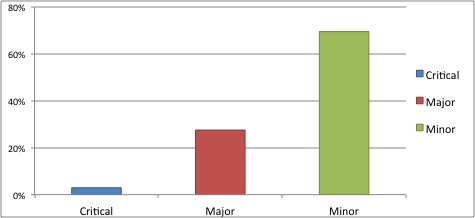
\includegraphics[width=\columnwidth]{graphs/graph1.jpg} 
\end{center}
\label{fig:defectimpact}
\end{figure}



TABLE I. 

\ \

\begin{tabular}{l*{2}{c}r} Severity & \% of Total \\ \hline Critical & 2.9\% \\ Major & 27.5\% \\ Minor & 69.5\%   \end{tabular}

\ \

Field defects were classified by impact, which are shown graphically in Fig. 1 and textually in TABLE I.  Shows the percentage of all defects of each severity type. The majority of defects found by the customer had a minor impact on their user experience (approximately 70\%), while approximately 28\% of users experienced a major severity defect and the remaining defects (just under 3\%) were of a critical severity.


\subsection{Defect Component}

In Fig. 2 we show the percentage of the total defects broken down by component and their severity. As we expect, in each component minor defects are the most common with critical defects being the least common

\begin{figure}[h]
\caption{\% Field defects by component and severity}
\begin{center}
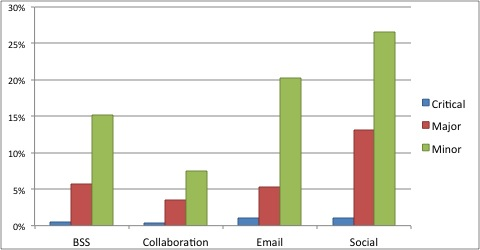
\includegraphics[width=\columnwidth]{graphs/graph2.jpg} 
\end{center}
\label{fig:defectcomp}
\end{figure}


TABLE II. 

\ \

\begin{tabular}{l*{5}{c}r} Severity & Critical & Major & Minor &  Total \\ \hline BSS & 0.5\%	& 5.7\% & 15.2\% & 21.4\% \\ Collaboration &	0.4\% & 3.5\% & 7.5\% & 11.4\% \\ Email	& 1.1\% & 5.2\% & 20.2\%	 & 26.5\%  \\  Social	& 1.0\% & 13.1\% & 26.5\% & 40.6\% \end{tabular}

\ \* 

TABLE II. Shows the percentage of all field defects broken down by component and severity. The Social application contained the most defects (41\%), The Email (27\%) and BSS (21\%) had a broadly similar level of defects, and while the collaboration application had the least percentage number of defects found with 11\%. Across all applications the customer was most likely to find a minor severity defect.

\ \*

\subsection{Data Centre Location}

In Fig. 3 below we show the percentage of the total defects broken down by Data Centre and severity. Again we expect, in each data centre that minor defects are the most common with critical defects being the least common. Previously we noted that both centres A and C are high usage, while data centre B is low usage. Given the level of field defects found in each data centre this supports the intuition that higher usage leads to a number of defects.

\begin{figure}[h]
\caption{\% Field defects by data centre and severity}
\begin{center}
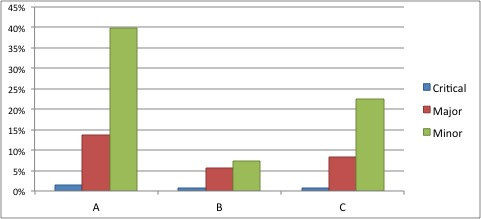
\includegraphics[width=\columnwidth]{graphs/graph3.jpg} 
\end{center}
\label{fig:defectdatacentre}
\end{figure}

TABLE III. 

\ \

\begin{tabular}{l*{5}{c}r} Data Centre & Critical & Major & Minor &  Total \\ \hline A & 1.6\%	 & 13.6\%	& 39.8\%	& 55.0\% \\ B & 0.7\% & 5.6\% & 7.3\% & 13.6\% \\ C	& 0.6\% & 8.3\% & 22.4\%	 & 31.3\%   \end{tabular}

\ \

TABLE III. Breaks down the Field defects by data centre and by severity.  55\% of all field defects found were in data Centre A. data centre C recorded 31\% of defects, while data Centre B recorded only 14\% of defects. 

\subsection{Defect Type}

In Fig. 4 below we show the percentage of the total defects broken down by testing type and severity. While we expect that minor severity would feature significantly, it?s interesting to observe that the majority of functional defects are minor in nature. Also we observe that for defects classified as System that the number of major and minor defects are practically the same. Finally we observed that in the case of Performance defects that the customer did not find very many. However of the defects that were found, slightly more were major severity.

\begin{figure}[h]
\caption{\% Field defects by test type and severity}
\begin{center}
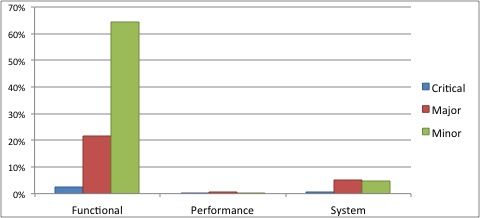
\includegraphics[width=\columnwidth]{graphs/graph4.jpg} 
\end{center}
\label{fig:defecttesttype}
\end{figure}

TABLE IV.

\ \ 

\begin{tabular}{l*{5}{c}r} Field Defect Type & Critical & Major & Minor &  Total \\ \hline Functional & 2.4\%	 & 21.8\%	& 64.3\%	& 88.5\% \\ Performance & 0.1\% & 0.7\% & 0.4\% & 1.2\% \\ System & 0.5\% & 5.0\% & 4.7\% & 10.3\%   \end{tabular}

\ \ 

We reviewed the percentage of field defects found according to their type. 89\% of all customer issues reported were functional in nature, a further 10\% of customer defects were related to end to end system issues, while only 1\% of defects found were related to performance of either client side user interface or underlying server system. 

\ \

\section{Discussion}

In section four we provided an outline of the field defects that were studied as part of our overall dataset, including defect impact, defect component, data centre location and defect severity. The following sections provide deeper analysis of our results. For each section we shall refer back to the research questions asked in section three.

\subsection{Defect Impact}

To answer how do field defects impact the customers? overall user experience, we can see clearly from both Fig. 1 and TABLE I, that the customer finds more minor defects than any other type, almost 70\%, which in real terms means that the customer will come across some unexpected behaviour which does not result in data loss during their day to day product usage. Given that minor severity defects are found most often, this supports that intuition that these types of defects are found by the customer exercising the most common component use cases. With the level of major defects found being 28\%, this also shows that these defects were found as part of a typical customers day to day usage albeit to a lesser degree than minor defects. Clearly as part of the customers typical use case, they did encounter some form of data loss or non-trivial unexpected behaviour. With approximately 3\% of field defects being critical, this suggests that the likelihood of a customer experiencing a total component or some system wide failure is a rare event. That said, customers either by themselves or in conjunction with other users were able to bring about behaviour, which impacted the wider system.
Given the nature of CD, it?s important to point that new code and features are released on a monthly basis. Therefore by it?s very nature new field defects are also raised on a continuous basis once new features are delivered. If a bug bounty program were introduced to incentivise field defect discovery, it would be interesting to determine the velocity of field defects from the introduction of such a scheme. Typically bug bounties have been the preserve of finding security defects, however by rolling out such a scheme for field defect discovery in general, it would be valuable to both the software developer: to focus on testing code paths which lead to higher severity issues, while incentivising the customer to uncover lower priority defects.

\subsection{Defect Component}

By examining defect location, we get a good indication of where customers find defects within the four main components. 
Fig. 2 and TABLE II highlight that at a component level approximately 41\% of the field defects found were in the social application a further 27\% found in the email application, with 21\% in the BSS component with a final 11\% found in the collaboration component. While defect yields may not map directly to application usage (No application usage metrics were available), we can look at the conditional probabilities to determine like likelihood of certain combination of defect attributes being found. We know what minor and major field defects were the most commonly found, so if we check for P(social\textbar minor), P(social\textbar major), P(email\textbar minor) and P(email\textbar major) we get probabilities of 0.3818, 0.4740, 0.2910 and 0.1901 respectively.  This tells us that the customer is more likely to find a social defect with either minor or major severity than any other component/impact combination. This supports the intuition that the more a component is used the more defects are likely to be found by end users.
In recent times social communication has become very popular. The high yield of social defects could be down to either user requirements or market demands for a rich social component feature set. We propose that for popular components (in our study social) that have continuous feature releases, by incentivising the discovery of lower impact defects by the customer, can help in-house testing refocus their efforts on the major severity testing across all test disciplines in their key feature/components areas. 

\subsection{Data Centre Location}
Fig. 3 and TABLE III give us an insight into how data centres are consumed by the customer. As mentioned in section III, we know that the level of usage varies from data centre to data centre, interestingly the customers of data centre A (High Usage) reported the highest number of field defects with 55\% while data centre C (Medium Usage) and data centre B (Low Usage) had 31\% and 14\% defects raised respectively. Clearly there may be some form of correlation between concurrent user population and field defects raised. 
Checking conditional probabilities for each data centre for both minor and major defects, as follows P(Minor\textbar DC-A) and P(Major\textbar DC-A) gives us 0.7236 and 0.2477 respectively. These conditionals tell us that we are more likely to find a minor defect within data centre A. For data centre B we checked the following conditions; P(Minor\textbar DC-B) and P(Major\textbar DC-B), which gives us 0.5368 and 0.4105 respectively. These conditionals tell a similar story to that of data centre A, that we are more likely to find a minor defect than a major one, however the distance between the probabilities is less pronounced. Finally checking P(Minor\textbar DC-C), P(Major\textbar DC-C) gives us 0.7140 and 0.2654 respectively. These conditional probabilities are very similar to those of data centre A. Customers are almost three times as likely to encounter a minor impact defect on data centre C than that of a major impact field defect.
Overall we found that that for high and medium usage data centres the likelihood of minor field defects was almost three times that of finding a major impact defect. For the low usage data centre the probability of finding a major impact field defect was broadly similar to that of finding a minor impact field defect.
In the context of CD, the same code is released to each data centre at the same time; clearly customers are more likely to be impacted differently depending on data centre. Knowing the underlying customer use cases is key at data centre level.
With knowledge of both data centre volume usage and with field defect data, incentivisation schemes can be tailor-made according to data centre. One obvious goal would be a bounty to flush out more minor field defects especially on the high usage data centres, while refocusing in-house resources to find more major impact defects prior to release. 

\subsection{Defect Type}
Finally we examine the defect type to understand which type of field defects that customer typically find. This metric alone may be one of the most important in terms of our findings, as it helps underscore which class of defect the end user is proficient at uncovering.
Fig 4 and TABLE III clearly indicate that functional defects are the most commonly uncovered by the customer with 89\% of all defects found being functional. Also of significance is the severity of these defects with 64\% being minor severity. Clearly functional defects typically present themselves in the form of user experience behaviour errors where the end user attempted an operation and the behaviour returned was unexpected. It?s also important to note that 10\% of all issues were system errors, typically these manifest themselves as expected behaviour during active concurrent usage. One can infer than system errors are less common than functional defects it may also be the case that system errors do not readily manifest themselves to the end user in the same way as functional defects.
Performance defects ranked the lowest in overall defects found with only 1\% of all problems being attributed to performance defects.  This data may suggest that either the performance of the components were adequately test prior to release or that performance defects may be harder for the end user to measure and quantify once in the field. 
Clearly from the customer?s perspective they are more likely to find functional defects as these issues typically manifest themselves within the UI, however the customer finds a greater proportion of lower impact functional defects. From a CD/CI perspective, a balance needs to be struck in terms of the features being released and their likely defect type yield. For backend server features in-house test teams can focus exclusively on Systems and Performance testing. For features with rich functionality in-house test teams can focus on use cases, which are likely to yield critical and major defects with some additional minor impact areas. 
In terms of bounties, for releases with high functional content software developers could award triple / double and single prizes for critical, major and minor impact field defects respectively with the knowledge that adequate testing would have been conducted in-house for critical and major use cases. Similarly for releases with high System and Performance and low functional features, proportional bounties may be awarded.


% An example of a floating figure using the graphicx package.
% Note that \label must occur AFTER (or within) \caption.
% For figures, \caption should occur after the \includegraphics.
% Note that IEEEtran v1.7 and later has special internal code that
% is designed to preserve the operation of \label within \caption
% even when the captionsoff option is in effect. However, because
% of issues like this, it may be the safest practice to put all your
% \label just after \caption rather than within \caption{}.
%
% Reminder: the "draftcls" or "draftclsnofoot", not "draft", class
% option should be used if it is desired that the figures are to be
% displayed while in draft mode.
%
%\begin{figure}[!t]
%\centering
%\includegraphics[width=2.5in]{myfigure}
% where an .eps filename suffix will be assumed under latex, 
% and a .pdf suffix will be assumed for pdflatex; or what has been declared
% via \DeclareGraphicsExtensions.
%\caption{Simulation Results}
%\label{fig_sim}
%\end{figure}

% Note that IEEE typically puts floats only at the top, even when this
% results in a large percentage of a column being occupied by floats.


% An example of a double column floating figure using two subfigures.
% (The subfig.sty package must be loaded for this to work.)
% The subfigure \label commands are set within each subfloat command, the
% \label for the overall figure must come after \caption.
% \hfil must be used as a separator to get equal spacing.
% The subfigure.sty package works much the same way, except \subfigure is
% used instead of \subfloat.
%
%\begin{figure*}[!t]
%\centerline{\subfloat[Case I]\includegraphics[width=2.5in]{subfigcase1}%
%\label{fig_first_case}}
%\hfil
%\subfloat[Case II]{\includegraphics[width=2.5in]{subfigcase2}%
%\label{fig_second_case}}}
%\caption{Simulation results}
%\label{fig_sim}
%\end{figure*}
%
% Note that often IEEE papers with subfigures do not employ subfigure
% captions (using the optional argument to \subfloat), but instead will
% reference/describe all of them (a), (b), etc., within the main caption.


% An example of a floating table. Note that, for IEEE style tables, the 
% \caption command should come BEFORE the table. Table text will default to
% \footnotesize as IEEE normally uses this smaller font for tables.
% The \label must come after \caption as always.
%
%\begin{table}[!t]
%% increase table row spacing, adjust to taste
%\renewcommand{\arraystretch}{1.3}
% if using array.sty, it might be a good idea to tweak the value of
% \extrarowheight as needed to properly center the text within the cells
%\caption{An Example of a Table}
%\label{table_example}
%\centering
%% Some packages, such as MDW tools, offer better commands for making tables
%% than the plain LaTeX2e tabular which is used here.
%\begin{tabular}{|c||c|}
%\hline
%One & Two\\
%\hline
%Three & Four\\
%\hline
%\end{tabular}
%\end{table}


% Note that IEEE does not put floats in the very first column - or typically
% anywhere on the first page for that matter. Also, in-text middle ("here")
% positioning is not used. Most IEEE journals/conferences use top floats
% exclusively. Note that, LaTeX2e, unlike IEEE journals/conferences, places
% footnotes above bottom floats. This can be corrected via the \fnbelowfloat
% command of the stfloats package.



\section{Conclusion}
Previous studies have shown that analysis of field defects is a valuable exercise. Additionally that bug bounty rewards provide an incentive to end users to improve software quality once in the field. The purpose of our study was to examine the role of the customer in the generation of field defects. We found that the customer was quite adept at finding minor severity functional defects. Also we found that the customer was less effective at finding higher severity performance and system defects irrespective of the data centre and application type used. The findings of this study support previous work particularly in the gaps between in-house software testing and general customer usage.
These findings provide a more detailed study in relation to software developed using a CD model. Adoption of CD means continuous feature releases and continuous defects, however feature releases can be delivered in such a away to ensure that there is not a significant burden on in-house test teams. 
 In future SME?s can assess their field defect data to understand the core gap areas in relation to defect impact, component, data centre and type. A specific test framework can then be built to allow SME?s to focus on test areas, which are likely to yield high impact defects, and which may be difficult for an end user to discover. 
Furthermore by providing the customer with an incentivised scheme in the form of bug bounties to find specific defects types will improve overall software quality through the iterative development and release process that is CD. 
In future work as CD gains more traction within the SME community we shall assess the framework behaviour in additional software domains such as mobile application development. 




% conference papers do not normally have an appendix


% use section* for acknowledgement
%\section*{Acknowledgment}


%The authors would like to thank...





% trigger a \newpage just before the given reference
% number - used to balance the columns on the last page
% adjust value as needed - may need to be readjusted if
% the document is modified later
%\IEEEtriggeratref{8}
% The "triggered" command can be changed if desired:
%\IEEEtriggercmd{\enlargethispage{-5in}}

% references section

% can use a bibliography generated by BibTeX as a .bbl file
% BibTeX documentation can be easily obtained at:
% http://www.ctan.org/tex-archive/biblio/bibtex/contrib/doc/
% The IEEEtran BibTeX style support page is at:
% http://www.michaelshell.org/tex/ieeetran/bibtex/
%\bibliographystyle{IEEEtran}
% argument is your BibTeX string definitions and bibliography database(s)
%\bibliography{IEEEabrv,../bib/paper}
%
% <OR> manually copy in the resultant .bbl file
% set second argument of \begin to the number of references
% (used to reserve space for the reference number labels box)
\begin{thebibliography}{1}

\bibitem{IEEEhowto:kopka}
Ec.europa.eu \emph{http://ec.europa.eu/growth/smes/business-friendly-environment/performance-review/files/annual-report/infographics\_en.pdf} Feb 2015

\bibitem{IEEEhowto:kopka}
J.  Humble  and  D.  Farley,  \emph{Continuous  Delivery:  Reliable  Software Releases  through  Build,  Test  and  Deplyment  Automation},  Addison-Wesley: Boston, 2011. 

\bibitem{IEEEhowto:kopka}
H. Holmstrom Olsson, H. Alahyari, and J. Bosch. Climbing the stairway to heaven":  A multiple-case study exploring barriers in the transition from agile development towards continuous deployment of software. In 38th \emph{Euromicro Conference on Software Engineering and Advanced Applications}, 2012

\bibitem{IEEEhowto:kopka}
Quora.com \emph{http://www.quora.com/What-are-the-best-examples-of-companies-using-continuous-deployment} Sept 2014.

\bibitem{IEEEhowto:kopka}
Wikipedia.org \emph{http://en.wikipedia.org/wiki/Bug\_bounty\_program} July 2015.

\bibitem{IEEEhowto:kopka}
Bugcrowd.com \emph{https://bugcrowd.com/list-of-bug-bounty-programs} 2015.

\bibitem{IEEEhowto:kopka}
Standford.edu \emph{http://www-cs-faculty.stanford.edu/~uno/} 2015. 

\bibitem{IEEEhowto:kopka}
Cr.yp.to \emph{http://cr.yp.to/djb.html} 2015.

\bibitem{IEEEhowto:kopka}
Brooks, P., Robinson, B., and Memon, A. M. An Initial Characterization of Industrial Graphical User Interface Systems. To appear in \emph{Proc. of the IEEE Int?l Conf on Software Testing, Verification, and Validation,} Apr 2009.

\bibitem{IEEEhowto:kopka}
Moritz, E.  Case study: how analysis of customer found defects can be used by system test to improve quality, in: \emph{31st International conference on, Software Engineering}, 2009, pp. 123?129

\bibitem{IEEEhowto:kopka}
Gittens, M., Lutfiyya, H., Bauer, M., Godwin, D., Kim, Y. W., and Gupta, P. An Empirical Evaluation Of System And Regression Testing. In \emph{Proc. of the Conf of the Centre For Advanced Studies on Collaborative Research,} pp. 3-15, 2002

\bibitem{IEEEhowto:kopka}
Musa, J. D., \emph{Software Reliability-Engineered Testing}, IEEE Computer , vol.29, no.11, pp.61-68, Nov 1996.

\bibitem{IEEEhowto:kopka}
Sullivan, M. and Chillarege, R., A Comparison of Software Defects in Database Management Systems and Operating Systems, In \emph{Proc. of Int\'l Symposium on Fault tolerant Computing,} pp. 475-484, July 1992.

\bibitem{IEEEhowto:kopka}
Adams, E. N.  \emph{Optimizing preventive service of software products.} IBM Journal of Research, 28(1), January 1984

\bibitem{IEEEhowto:kopka}
Software Engineering Standards Committee, \emph{IEEE Recommended Practice for Software Requirements Specifications,} The Institute of Electrical and Electronics Engineers, IEEE Std. 830-1998, 1998.

\end{thebibliography}

% that's all folks
\end{document}

